\documentclass[a4paper]{article}
\usepackage[spanish]{babel}
\usepackage[utf8]{inputenc}
\usepackage{fancyhdr}
\usepackage{charter}   % tipografía
\usepackage{graphicx}
\usepackage{makeidx}

\usepackage{float}
\usepackage{amsmath, amsthm, amssymb}
\usepackage{amsfonts}
\usepackage{sectsty}
\usepackage{wrapfig}
\usepackage{listings} % necesario para el resaltado de sintaxis
\usepackage{caption}

\usepackage{hyperref} % agrega hipervínculos en cada entrada del índice
\hypersetup{          % (en el pdf)
    colorlinks=true,
    linktoc=all,
    citecolor=black,
    filecolor=black,
    linkcolor=black,
    urlcolor=black
}

\usepackage{color} % para snippets de código coloreados
\usepackage{fancybox}  % para el sbox de los snippets de código

\definecolor{litegrey}{gray}{0.94}

% \newenvironment{sidebar}{%
% 	\begin{Sbox}\begin{minipage}{.85\textwidth}}%
% 	{\end{minipage}\end{Sbox}%
% 		\begin{center}\setlength{\fboxsep}{6pt}%
% 		\shadowbox{\TheSbox}\end{center}}
% \newenvironment{warning}{%
% 	\begin{Sbox}\begin{minipage}{.85\textwidth}\sffamily\lite\small\RaggedRight}%
% 	{\end{minipage}\end{Sbox}%
% 		\begin{center}\setlength{\fboxsep}{6pt}%
% 		\colorbox{litegrey}{\TheSbox}\end{center}}

\newenvironment{codesnippet}{%
	\begin{Sbox}\begin{minipage}{\textwidth}\sffamily\small}%
	{\end{minipage}\end{Sbox}%
		\begin{center}%
		\colorbox{litegrey}{\TheSbox}\end{center}}



\usepackage{fancyhdr}
\pagestyle{fancy}

%\renewcommand{\chaptermark}[1]{\markboth{#1}{}}
\renewcommand{\sectionmark}[1]{\markright{\thesection\ - #1}}

\fancyhf{}

\fancyhead[LO]{Sección \rightmark} % \thesection\
\fancyfoot[LO]{\small{Camila Coy, Uriel Fadel, Jorge Porto, Carlos Soliz}}
\fancyfoot[RO]{\thepage}
\renewcommand{\headrulewidth}{0.5pt}
\renewcommand{\footrulewidth}{0.5pt}
\setlength{\hoffset}{-0.8in}
\setlength{\textwidth}{16cm}
%\setlength{\hoffset}{-1.1cm}
%\setlength{\textwidth}{16cm}
\setlength{\headsep}{0.5cm}
\setlength{\textheight}{25cm}
\setlength{\voffset}{-0.7in}
\setlength{\headwidth}{\textwidth}
\setlength{\headheight}{13.1pt}

\renewcommand{\baselinestretch}{1.1}  % line spacing


\usepackage{underscore}
\usepackage{caratula}
\usepackage{url}
\usepackage{color}
\usepackage{clrscode3e} % necesario para el pseudocodigo (estilo Cormen)

%\usepackage{algorithm}
%\usepackage{algorithmic}
\usepackage{algorithm}[1]
\usepackage{algorithmic}[1]
%\usepackage{algpseudocode}

\definecolor{dkgreen}{rgb}{0,0.6,0}
\definecolor{gray}{rgb}{0.5,0.5,0.5}
\definecolor{mauve}{rgb}{0.58,0,0.82}

\lstset{frame=tb,
  language=JAVA,
  aboveskip=3mm,
  belowskip=3mm,
  showstringspaces=false,
  columns=flexible,
  basicstyle={\small\ttfamily},
  keywordstyle=\color{blue},
  commentstyle=\color{dkgreen},
  stringstyle=\color{mauve},
  breaklines=true,
  breakatwhitespace=true,
  tabsize=3,
  numbers=left,
  xleftmargin=2em,
  frame=single,
  framexleftmargin=2em,
  numbersep=5pt,                   % how far the line-numbers are from the code
  numberstyle=\small\color{gray} % the style that is used for the line-numbers
 }

\begin{document}


\thispagestyle{empty}
\materia{Algoritmos y estructuras de dato III}
\submateria{Segundo Cuatrimestre de 2015}
\titulo{Diseño  y técnicas de algoritmos}
\subtitulo{Aplicacion de técnica}
\integrante{Coy, Camila Paula}{33/14}{camicoy94@gmail.com} % por cada integrante (apellido, nombre) (n° libreta) (e-mail)
\integrante{Fadel, Uriel}{104/14}{urielfadel@gmail.com}
\integrante{Porto, Jorge}{376/11}{cuanto.p.p@gmail.com}
\integrante{Soliz, Carlos}{406/12}{rcarlos.cs@gmail.com}

\maketitle
\newpage

\thispagestyle{empty}
\vfill

\thispagestyle{empty}
\vspace{1.5cm}
\tableofcontents
\newpage

%\normalsize

\newpage
\section{Objetivos generales}

El objetivo del siguiente trabajo sera la practica de dístintos técnicas para elaboracion de algoritmos.
Tal trabajo consta de tres situaciones que bien pueden ser aplicadas a la vida real. 
Uno de los cuales se resolvera aplicando un algoritmo golozo, otros
utilizaran estructuras de datos eficiente para lograr el objetivo de performance y como ultima tecnica algoritmica se hara uso de backtraking
con la meta de obtener la solucion deseada.  
%\newpage



%\newpage
\section{Problema 1}
\subsection{Descripción del problema.}

\vspace*{0.3cm}



\textbf{Introduccion al problema} \newline

Como es sabido en la Republica Argentina y talvez otros paises, las sistema ferreo esta distribuido en forma de abanico como en la \textbf{figura 1}.
En el ejemplo de abajo tenemos todas las lineas ferroviarias, tienen como origen la Capital Federal.
\begin{figure}[htb]
	\begin{center}
		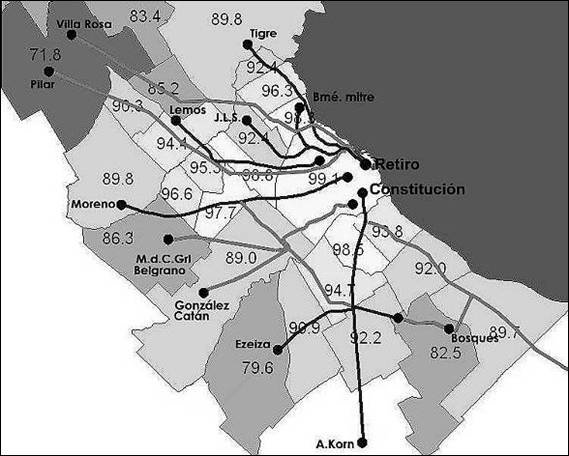
\includegraphics[scale=0.50]{imagenes/red-trenes.jpg}
	\end{center}
	\caption{Trenes provincia de Buenos Aires, Argentina}
\end{figure}
Y cada linea ferroviarria tiene una estacion inicial y las estaciones que le siguen a la inicial. Como por ejemplo en la \textbf{figura 2}, donde la estacioon inicial Retiro, Saldias, ... , Villa Rosa. 
Cada estacion esta ubicada una cierta distancia respecto de la estacion inicial.
Por ejemplo:

\begin{figure}[htb]
	\begin{center}
		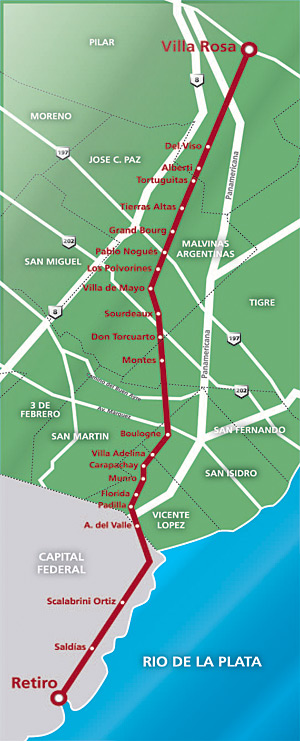
\includegraphics[scale=0.25]{imagenes/Belgrano-Norte.jpg}
	\end{center}
	\caption{Linea de tren Belgrano Norte}
\end{figure}

Cada estacion esta ubicada una cierta distancia respecto de la estacion inicial.
Por ejemplo:
\begin{center}
   \begin{tabular}{ | l | c | r | }
     \hline
     estacion & distancia a estacion Retiro \\ \hline
     Retiro  & 0 \\ \hline
     Saldias  & 5\\ \hline
     Scalabrini Ortiz & 10 \\ \hline
     Aristobulo Del Valle & 14 \\ \hline
     ... & ... \\ \hline
     Villa Rosa & 60 \\ 
     \hline
   \end{tabular}
\end{center}

\textbf{Problema concreto} \newline

Nos han encomendo el trabajo de conectar telegraficamente todas las estaciones del sistema ferreo,
para cada linea del sistema ferreo se le destinara una cantidad en metros de cable y deberemos conectar maxima cantidad posible de estaciones. Dicho cable no debera cortarse, sino que su uso con el cable entero.

Este es un tipico problema de optimizacion en este caso de trata de una maximizacion.
El objetivo nuestro es la busqueda de un algoritmo que pueda conectar la mayor cantidad de estaciones de una linea ferrea con el uso de un solo cable de determinada longitud.  

Nuestro input esta compuesta por la primer linea donde se indica la longitud de cable destinada para esa linea ferrea. La siguiente linea seran una serie 
de numeros separados por un espacio y ordenados de manera no decreciente (osea estrictamente creciente), donde cada numero representa la distancia hacia la $estacion_0$. 
Respecto a la serie de numeros:
\begin{itemize}
    \item La $estacion_0$ no esta en la serie pues su distancia hacia si misma es $0$.
    \item la serie comienza con la distancia de la $estacion_1$, $estacion_2$, ...., $esta4cion_n$, todas las distancia son respecto a la $estacion_0$ 
\end{itemize}

\textbf{Ejemplo input y sus respectivos output: } 

\begin{center}
   \begin{tabular}{ | l | c | r | }
     \hline
     longitud cable(input) & distancias de estaciones(input) & maxima cantidad de ciudades (output)\\ \hline
     4 & 1 4 6 7 8 9 & 4 \\ \hline
     2 & 1 2 3 4 5 6 7 & 3 \\ \hline
     7 & 1 2 3 4 5 6 7 & 8 \\ \hline
     2 & 4 8 15 & 0 \\
     \hline
   \end{tabular}
\end{center}


%	\begin{figure}[htb]
%  \begin{center}
%      \includegraphics[scale=0.25]{imagenes/red-ferroviaria.jpg}
%	  \end{center}
% \caption{ejemplo}
%\end{figure}

\newpage
\subsection{Desarrollo de la idea y pseudocódigo.}

\vspace*{0.3cm}

%\textbf{completar.}
\textbf{}
Para el desarrollo de nuestro algoritmo pusimos todas distancias de las estaciones en un arreglo en el orden en que venian i ademas agregamos la estacion_0 con distancia 0, la longitud del cable fue almacenada en un entero.
 
Nuestro algoritmo utiliza un bucle principal el cual podria iterar $n$ veces, y cada itercion verifica que no nos hayamos pasado de longitud del arreglo.
Para el controlar las la cantidad de iteraciones que hacemos usamos dos variables que vamos a llamar $desde$ y $hasta$, donde estas variables marcar en que subarreglo estamos ubicados. En cada iteracion lo que hacemos es empezar a contar las ciudades desde donde dejamos $desde+1$ y $hasta-1$, esto me asegura que itere solamente n veces. De ahi que vamos a llega deducir que el algoritmo en lineal al tamanio de la entrada. 


\textbf{pseudocodigo} \newline 

\begin{codebox}
\Procname{$\proc{maximasEstacionesConectadas}(array<int> \ estaciones,Nat \ mCables)	$}
	\li inicializamos las variables enteras $desde$,$hasta$,$cantEstacionesConectadas$,$cantidadDeEstacionesMaxima$ en 0.
	\li inicializamos las variables booleana $mePase$ en $false$.
	\li \While $(hasta < estaciones.length -1)$
	\li \Do	 // veo cuantas estaciones pudo unir con el cable.
		\li \While ($hasta<estaciones.length \land estaciones[hasta]-estaciones[desde]<=mCable$) 
		\li \Do	
				\li $hasta++$ // porque agregamos una estacion mas
				\li $mePase \leftarrow true$.
			\End
			\li \If $mePase$ 
			\li \Then 
					$hasta \leftarrow hasta-1;$
					$ mePase \leftarrow False;$
			\End		
			\li $cantEstacionesConectadas$ es Cero si $desde==hasta$ , sino $hasta-desde + 1$
			\li $cantidadDeEstacionesMaxima \leftarrow$ Max( $cantidadDeEstacionesMaxima$,$cantEstacionesConectadas$);
			\li $desde \leftarrow desde+1$  
		\End	
	\End
	\li \Return $\id{cantidadDeEstacionesMaximas}$ // retorno la mayor cantidad de estaciones que se pudieron conectar
	      
\end{codebox}

\newpage
\subsection{Justificación de la resolución y demostración de correctitud.}

\vspace*{0.3cm}

\textbf{Teorema: } El algoritmo golozo utilizado encuentra siempre una solucion optima (donde solucion optima se refiere a conectar la mayor cantidad de estaciones posible).

\textbf{Demostracion: } Probaremos que dada una solucion optima $S$, el algoritmo genera una solucion $S'$ con por lo menos la misma cantidad de estaciones que la solucion $S$, es decir que la solucion generada por el algoritmo golozo es optima. \newline
Supongamos por el \underline{absurdo} que la solucion $S'$ dada por el algoritmo golozo no es optima y tomaremos la solucion optima $S$ que mas estaciones comparta con con la solucion brindada por el algoritmo golozo $S'$.
\newline
por ejemplo: $estaciones = \{x_1 x_2 x_3 x_4 x_5 x_6 x_7 \}$ ,  $S =\{ x_2 x_3 x_4 x_5 x_6\}$  y  $S'=\{ x_2 x_3 x_4 x_5\}$.  
\newline
Sean $S$ el secuencia de solucion optima y $S'$ la secuencia brindada por el algoritmo golozo.
Supongamos ademas que ambas secuencas tienen el mismo origen (osea, $S_1$ == $S'_1$).
Sea $S_j$ el primer elemento distinto del los elementos de $S'$ ($S_j$ existe pues supusimos que $S'$ no optimo), en pocas palabras 
para todo $i<j$ vale $S_i = S'_j$. De esta manera sabemos que podemos conectar $S_{j-1}$ con $S_{j}$ pues es solucion optima.
Pero entonces $S'_j$ es elegido por nuestro algoritmo como elemento que se conecta con $S'_{j-1}$, entonces debe suceder que $S_j = S'_j$.
Pero llegamos a que $S = S'$ comparten todos los puntos entonces llegamos a que $S'$ es optimo absurdo.\newline
El absurdo viene de supóner que $S'$ no es optimo.   	



%\newpage
\subsection{Análisis de complejidad propuesta.}
La complejidad de mi algoritmo es $O(n)$, pero al tener dos ciclos anidados. No esta demas decir que  en ambos ciclos realizamos operaciones que cuestan $O(1)$,  ya que son operaciones aritmeticas(sumas, restas), asignaciones.
Como se desprende del pseudocodigo que como mucho el ciclo mayor(linea 3 pseudocodigo)va ciclar n veces y como poco cicla 1 ves.
 Veamos algunos casos:  
 \begin{itemize}
    \item Caso en el que el ciclo mayor cicla 1 vez, dentro del ciclo mayor tenemos un ciclo menor(linea 5 pseudocodigo) que ciclara la $n-1$ veces que me faltan ciclar y con esto ya tendiramos las n iterciones. Ejemplo de esto seria por ejemplo que el cable pudiera conectar a todas las estaciones ($estaciones=\{1,2,3,4,5,6\})y$ $mCable= 6$).
    \item El caso en que el ciclo mayor cicla n veces pordria ser por ejemplo que no podamos conectar niguna ciudad, por lo tanto el ciclo menor costaria $O(1)$ y el ciclo mayor ciclaria $n$ veces. Ejemplo: $estaciones = \{4,8,12\}, mCable = 3$, como vemos no podemos conectar ninguna estacion,
    \item Hay casos intermedios que son de  similar analisis.
\end{itemize}

Podemos deducir que la complejidad de el algoritmo es $O(n)$, ya que los dos ciclos estan interrelacionados, la variable ''hasta'' solo puede llegar a n. Para el ciclo anidado mas externo en cada iteración, incrementa la variable ''hasta'' una cierta cantidad de veces, finalmente incrementa la variable ''desde''. Aunque solo se incremente una o cero veces la variable ''hasta'', lo estará haciendo la variable ''desde'', y como siempre ''desde'' $ \leq $ ''hasta'', tenemos a lo sumo n incrementos para la variable ''desde'' y n para ''hasta''.
 

\subsection{Experimentación y gráfico.}

\vspace*{0.3cm}
En las secciones anteriores nos ocupamos de la complejidad teorica.
Ahora lo que nos interesara  es contrastar lo teorico con lo experimental, lo haremos haciendo experimento, los cuales plasmaremos en un grafico. 
Como ya habiamos comentado en la parte de analisis de complejidad, nuestro algoritmo teoricamente no tiene un peor y mejor. Por consiguiente(caso peor, mejor, aleatorio) los graficos seran todos similares entre si.   

\begin{figure}[htb]
  \begin{center}
      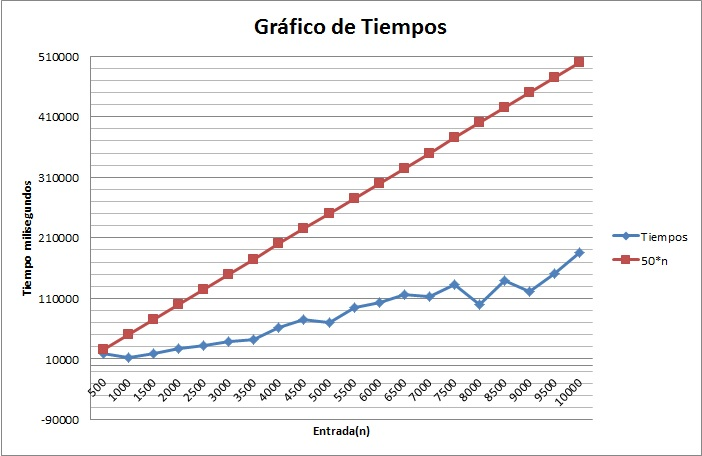
\includegraphics[scale=0.75]{imagenes/GraficoEj1.jpg}
  \end{center}
  \caption{ejemplo}
\end{figure}


Para tomar los tiempos utilizamos instancias de tamaños entre 500 a 10000 elementos. 
Lo que hicimos fue para cada instancia correr 200 veces el algoritmo golozo y tamamos el promedio de los resultados que tuvieran una variación estándar.
Para hacer esto filtramos los tiempos y nos quedamos con aquellos que estubieran entre el promedio menos el desvío estándar y promedio mas el desvío estándar.El desvío estándar mide cuanto tienden a alejarse los resultados del promedio. Para calcular el desvío, primero tuvimos que calcular la varianza. Para obtener la varianza agarramos cada uno de los tiempos y  les restamos el promedio y lo elevamos al cuadrado, después tomamos el promedio de esos resultados. Para terminar de calcular el desvío solo sacamos la raíz cuadrada de la varianza. Para hacer esto
\newline
Como podemos apreciar en el gráfico nuestro  algoritmo tiende a tener una complejidad exactamente lineal, ya que a simple vista la podemos acotar superiormente e inferiormente por n. \newline
\textbf{Observación: } utilizamos el desvío estándar porque la computadora puede tardar mucho mas o mucho menos, lo que haces es tomar el promedio de las cosas que no se va muy por fuera de lo esperado
	


%\newpage
%\subsubsection{Test 2}

%\vspace*{0.3cm}

%\textbf{completar!}


%\newpage
%\subsubsection{Test 3}

%\vspace*{0.3cm}

%\textbf{completar!}


\newpage
\section{Problema 2}
\subsection{Descripción del problema.}

\vspace*{0.3cm}
\textbf{Introduccion} \newline
Como muchos saben en el ambito de las estadisticas, la mediana representa el valor de la variable en posicion central en un conjunto de datos ordenado.
Existen varios metodos para el calculo de la mediana, pero uno de los mas conocidos el siguiente.
Sean $\{x_1,x_2,x_3,...,x_n\}$ ordenadas en orden creciente, llamaremos $M_e$ a mediana del conjunto, pueden haber dos caso:

\begin{itemize}
    \item Si $n$ es impar, la mediana el valor ocupado en la posicion $(n+1)/2$, osea $M_e = x_{(n+1)/2}$.
    Ejemplo: tenemos 5 elementos ordenados $\{ 3,6,7,8,9 \}$ el valor central es el tercero, la mediana es elemento $M_e = 7$
    \item Si $n$ es par, la mediana es la suma de los elemento ocupados en la posicion $i/2$ y $i/2+1$ y luego dividir ese valor por 2, osea $ M_e = (x_{n/2} + x_{(n/2+1)})/2$.
    Ejemplo: Tenemos 6 datos ordenados $\{ 3,6,7,9,10,11 \}$ los dos valores para calcular la mediana son los $x_3=7$ y $x_4=9$, $ M_e = (7+9)/2 = 8$. 
\end{itemize}
En la \textbf{figura 3} tenemos unos graficos con las diferencias entre moda, mediana y media de una funcion arbitraria de densidad de probabilidad.	  
\begin{figure}[htb]
	\begin{center}
		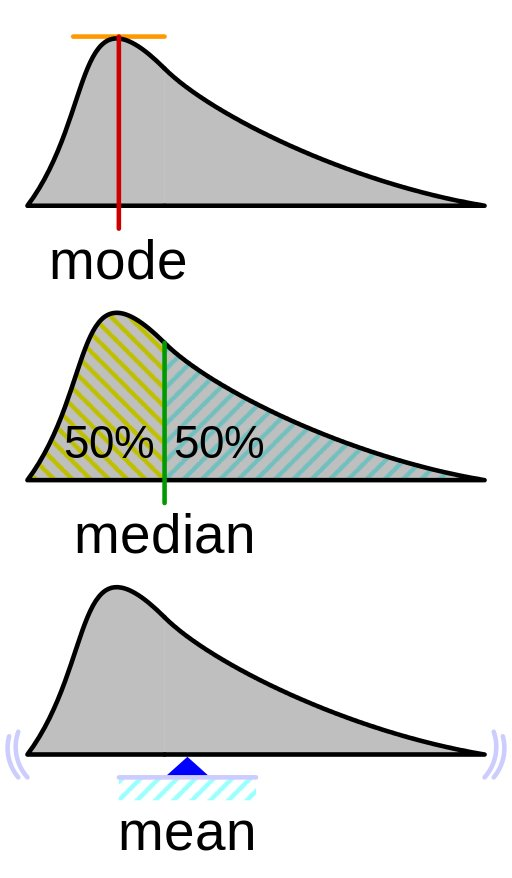
\includegraphics[scale=0.25]{imagenes/mediana.jpg}
	\end{center}
	\caption{Imagenes de la moda, mediana, media}
\end{figure}

\textbf{Problema} \newline

En nuestro problema nos han encomendado calcular y guardar las medianas parciales de una secuencia de numeros que no tine ningun orden fijo. \newline
Como por ejemplo: Nuestro secuencia de datos entrada(input) son \textbf{\{1,5,2,7,10\}}, las salida(output) debe ser \textbf{\{1,3,2,3,5\}},
en el cuadro de abajo los numeros marcados en negro son los numeros con los que calculo la mediana en ese instante. 

\begin{center}
   \begin{tabular}{| l | c | r | r |}
     \hline
     Nro de iteracion & 5 Nros entero(input)  &  Mediana en actual iteracion & Construccion de la secuencia solucion \\ \hline
     1 & \textbf{1} 5 2 7 10  & 1 & 1 \\ \hline 
     2 & \textbf{1 5} 2 7 10  & 3 & 1 3 \\ \hline 
     3 & \textbf{1 5 2} 7 10  & 2 & 1 3 2 \\ \hline 
     4 & \textbf{1 5 2 7} 10  & 3 & 1 3 2 3\\ \hline 
     5 & \textbf{1 5 2 7 10}  & 5 & 1 3 2 3 5\\ \hline 
     \hline
   \end{tabular}
\end{center} 

Veamos mas especificamente que quier decir el cuandro:.

\begin{itemize}
    \item En la itercion_1 calculo la mediana solamente con el elemento $1$,la mediana en ese instante es el $1$, mi secuencia solucion parcial queda $\{1\}$.
    \item En la itercion_2 calculo la mediana solamente con los elemento $\{1,5\}$, la mediana en ese instante es el $3$, mi secuencia solucion parcial queda $\{1,3\}$.
    \item En la itercion_3 calculo la mediana solamente con los elemento $\{1,5,2\}$, la mediana en ese instante es el $2$, mi secuencia solucion parcial queda $\{1,3,2\}$.
	\item y asi hasta llegar a la $5-esima$ iteracion, por consiguiente a la solucion.
\end{itemize}
%\begin{figure}[htb]
%  \begin{center}
%      \includegraphics[scale=0.25]{imagenes/ejemplo.jpg}
%  \end{center}
%  \caption{ejemplo}
%\end{figure}



\newpage
\subsection{Desarrollo de la idea y pseudocódigo.}

\vspace*{0.3cm}






Despues de cada numero de entrada se tiene que calcular la mediana en base a los numeros leidos hasta el momento,
entonces cuando llegamos al 1, solo tenemos a ese numero, y le resto de la secuencia no importa en el momento, entonces la secuencia de salida,
osea el secuencia de las medianas, se sabe que el i-esimo numero de la secuencia de salida, es la mediana, calculada entre el primer numero y el
i-esimo numero de entrada.

Entonces en base a ese problema, y que necesitamos tener un orden menor a $n^2$, encontramos una 
solucion que abarca una estructura de datos conocida, como es el Heap. En esta solucion usaremos dos heaps, uno ordenado de manera creciente,
y la otra de manera decreciente. Cuando hablo de manera creciente me refiero a que la raiz va a ser el menor numero, y que hacia abajo va a ir
teniendo numeros mayores o iguales. Ademas de usar 2 heaps para nuestra solucion, tambien estaremos usando un invariante entre estos dos heaps,
que tiene que cumplir, que en uno van a estar los numeros menores, y en el otro los mayores, y ademas de esto, otro invariante que el cardinal
de ambos no pueden tener una diferencia mayor a 1. Este invariante se usara para lograr calcular la mediana de forma rapida, ya que al tener el 
invariante de cardinalidad, sabemos que si uno de los dos tiene mayor cantidad de elementos, entonces su elemento, mayor o menor dependiendo de 
cual heap hablamos va a ser la mediana hasta ese momento, y si tienen la misma cardinalidad, va a ser el promedio de los dos numeros que 
predominan en cada uno de los heaps. Y esto se cumple solo porque esta el primer invariante de que en uno de los heaps estan los menores y en 
el otro los mayores.
Tambien tengo que aclarar que el heap de los numeros menores, va a tener a su mayor numero de raiz del heap, (osea como primer elemento), y que 
los numeros mayores van a tener a su menor elemento. En el codigo, de la solucion, la manera de mantener el invariante de que estan separados por
mayor y por menor, los heaps, se lo asegura jugando con el segundo invariante de cardinalidades. Se dice que cuando se tiene que agregar un numero
a un heap que tiene antes de agregarle, mas elementos que el otro, entonces hay que sacarle el primero( con primero me refiero a raiz de ese heap)
y pasarle ese numero al otro heap, y luego agregarle ese numero. De esta manera siempre se mantienen ambos invariantes, y para saber si se deberia
agregar en uno de los heaps o en el otro simplemente se fija, si el elemento a agregar, es mayor al menor de los mayores, o menor al mayor de
los menores.




\newpage
\subsection{Justificación de la resolución y demostración de correctitud.}

\vspace*{0.3cm}

%\textbf{completar!}
A continuacion vamos a justificar, porque se cumple el funcionamiento de el ejercicio 2.
Como hemos explicado anteriormente, tenemos dos colasPrioridad, que cumplen dos invariantes. HeapMenores, va a ser la ColaPrioridad que contenga a los elementos mas chicos leidos hasta el momento, y el HeapMayores va a ser la ColaPrioridad que contenga a los elementos mas grandes, leidos hasta el momento. \newline 

\textbf{Invariante: }
\begin{itemize}
    \item La cardinalidad de ambos, no tienen una diferencia mayor a 1. Con su cardinalidad me refiero a la cantidad de elementos que cada uno de las ColaPrioridad. %Desde ahora $#(HeapMenores)$ y $#(HeapMayores)$.
    \item El elemento mayor de la ColaPrioridad de los menores, va a contener un elemento, que sea menor o igual, al elemento menor del heap de los mayores.
\end{itemize}

En base a esto sacamos la conclucion de que, si la cardinalidad de ambas ColasPrioridad, son iguales, y son distintos de cero, entonces la cantidad de elementos es una cantidad par, por ende, segun la definicion de mediana, la mediana es el promedio de los dos elementos de los numeros ordenados, leidos hasta el momento. \newline
Y que si la cardinalidad es distinta, entonces la cantidad total de elementos leidos es impar, (esto se puede ver por el invariante de la diferencia), ya que: \newline

Si n es par, n+(n+1), es impar, ya que 2n es par, y un $par + 1$ es impar. \newline
Y lo mismo con n+(n-1), ya que 2n es par y un par -1 es impar.	\newline

Entonces por la definicion de mediana, la mediana es el elemento del medio de los numeros ordenados.

Ahora se analizara porque se cumple que el elemento del medio, en caso de que la cardinalidad total es impar, es el elemento primero, de la colaPrioridad que tenga la mayor cardinalidad.

Si miranmos una secuencia de numeros ordenados se va a poder ver claramente:
Supongamos que tengo la secuencia $\{1,2,3,4,5,6,7,8,9\}$, se puede ver que es el elemento $5$ es la mediana. \newline
Si se lo divide por menores y por mayores.

Por un lado tenemos los menores: $\{1,2,3,4\}$ y por otro los mayores, $\{6,7,8,9\}$
y luego el elemento del medio que podria ir en cualquiera de los dos. Por nuestra forma de implementarlo va a ir con los menores.
Entonces los menores, serian: $\{1,2,3,4,5\}$ y no solo que el 5 esta ahi, sino que es el elemento mayor, de los numeros chicos.
Si pondriamos al 5, con los mayores, este elemento seria el menor de ellos.
Nuestras ColasPrioridad estan ordenados de la siguiente manera: La ColaPrioiridad de los menores, tiene como primer elemento, al mayor. Y la ColaPrioridad de los mayores, tiene como primer elemento al menor.

Entonces si partimos una secuencia ordenada en dos partes iguales, los elementos del medio serian, el ultimo de la primera mitad, y el primero de la segunda, y esto es justamente lo que pasa con las ColasPrioiridad.
La ColaPrioiridad es nuestra forma de mantener ordenados los elementos, y el invariante de que su cardinalidad no tenga una diferencia mayor a 1, es la forma que hacemos para poder identificar rapido al elemento mediano.

Y la razon de que el elemento mediano es el primero(con primero revisar como esta hecha la ColaPrioridad) del que tenga mayor cardinalidad es porque:

Si tenemos n elementos, con n impar. Una ColaPriorodad va a contener (n-1)/2 elementos, y la otra (n-1)/2 + 1.
Podemos ver facilmente que si tenemos una secuencia de enteros ordenada, si vamos quitando el mayor y el menor cada vez, el elemento restante va a ser el elemento mediano.\newline
Vease este ejemplo simple:
Tengo la secuencia $\{1,2,3,4,5\}$  saco 1,5 $\rightarrow$  $\{2,3,4\}$  saco 2,4 $\rightarrow$ $\{3\}$ que es la mediana. \newline
Una vez que termina de recorrer todos los elementos de la entrada ,ahi el algoritmo devolvera la solucion(secuencia de medianas) y terminara.

\newpage
\subsection{Análisis de complejidad.}

\vspace*{0.3cm}

%\textbf{completar!}
Ahora que la forma de la solucion esta explicada, vamos a pasar a demostrar como es que cumple el orden de complejidad, menor a $n^2$.
Al tener dos conjuntos, basados en heap, y buscando en como esta implementado el heap que usamos de java, este explica que el orden cumple de 
agregar elementos en log $O(n)$, eliminar el primer elemento en $O(log(n))$, hacer un peek al primer elemento en $O(1)$ y buscar un elemento en $O(n)$,
pero esto no lo  hacemos nunca, porque no nos interesa todos los elementos en cada momento sino los primeros de cada heap.
\newline
Basandonos en que los heaps cumplen este orden pasamos a demostrar que nuestro codigo tambien cumple con este orden:
Nuestro codigo tiene un estilo de $while$, que es el que va a ir agarrando los numeros 1 por 1, esto se podria contar como un while de n numeros
suponiendo que n cumple que es la cantidad de numeros de entrada. Y luego, tiene los ifs correspondientes que son para verificar en cuales de
los casos explicados anteriormente cae el numero de entrada. Pero todo lo que hace en cada uno de los ifs, o el else, son simplemente verificar
en que caso cae que eso se cumple en $O(1)$ ya que son comparar numeros enteros, y luego en el peor de los casos tiene que sacar el primer elemento
de uno de los heaps (que eso se hace en $log (n)$ ) luego agregarlo en el otro heap (otro $log(n)$) y luego agregar ese elemento en su heap 
correspondiente ($log(n)$). Y esto cumple un orden de $3*(log(n))$ y si asumimos que el while es n veces, entonces son $3*n*log(n)$ que esta incluido
en el orden de $n*log(n)$. Y esto es exagerando un poco en realidad, porque cada uno de los heaps puede contener como mucho no $n$, sino $i/2$ elementos
con $i$ siendo la cantidad de numeros que ya leimos hasta el momento. Entonces en realidad el peor orden que puede tener nuestro ejercicio, 
es que siempre cuando son impares nuestro elemento caiga en el peor caso, que seria el de $3*log(i/2)$.



Entonces el peor caso es:

$ O(\sum_{i=1}^{n}3*log(i+1/2) + \sum_{i=1}^{n}3*log(i/2))= O(n*log(n)+3*n(log)) = O(n*log(n))$.

Que exagerando a los i por n, nos queda en el orden de $n*log(n)$.



\newpage
\subsection{Experimentación y gráficos.}

Para generar las instancias de toma de tiempos del problema 2 lo que hacemos es generar numeros aleatorios e ir guardandolos en un array hasta que este se llene, el tamaño del array se define segun el tamaño de la instancia que se quisiera. En el caso de lo que se quisiera fuera un peor caso, se generan numeros aleatorios, se le suma el anterior y se guarda en el array, ya que el peor caso es que los numeros vengan en forma creciente, teniedolos que guardar siempre en el heap de los mayores. Para en mejor caso se miraba cual tenia mas y se generaba un numero aleatorio que entrara en el heap de menor cantidad, si habia menos mayores se generaba un numero menor al minimo de los mayores y sino se generaba un numero y se le sumaba el mas grande de los chicos. En el caso de que tuvieran la misma cantidad se genera uno aleatorio y se guarda donde corresponda, en caso de que este entre el menor de los mayores y el mayor de los menores pasa a ser el mas grande de los menores. Para esto utilizamos la clase $ GeneradorInstancias $.

Se toman los tiempos igual que para el problema 1.
%Para tomar los tiempos pasamos 200 veces el mismo input(en el caso del ejercicio 3 hay que poner: pasamos 50 veces el mismo input, ya que tarda mucho en ejecutarse el programa con e grandes), y tomamos el promedio de los resultados que estuvieran un variacion estandar. Para ello filtramos los tiempos y nos quedamos con aquellos que estuvieran entre el promedio menos el desvio estandar y promedio mas el desvio estandar. El desvio estandar mide cuanto tienden a alejarse los resultados del promedio. Para calcular el desvio, primero tuvimos que calcular la varianza. Para obtener la varianza agarramos cada uno de los tiempos y  les restamos el promedio y lo elevamos al cuadrado, despues tomamos el promedio de esos resultados. Para terminar de calcular el desvio solo sacamos la raiz cuadrada de la varianza. Para esto utilizamos la clase $ Tiempos $.
%En el problema 1 se genero una secuencia de numeros aleatorios creciente, igual que en el peor caso del problema 2. dejando el tamaño del cable constante ya que este no afecta para las mediciones.


 En los siguientes gráficos tenemos los resultados obtenidos.

\begin{figure}[H]
  \begin{center}
      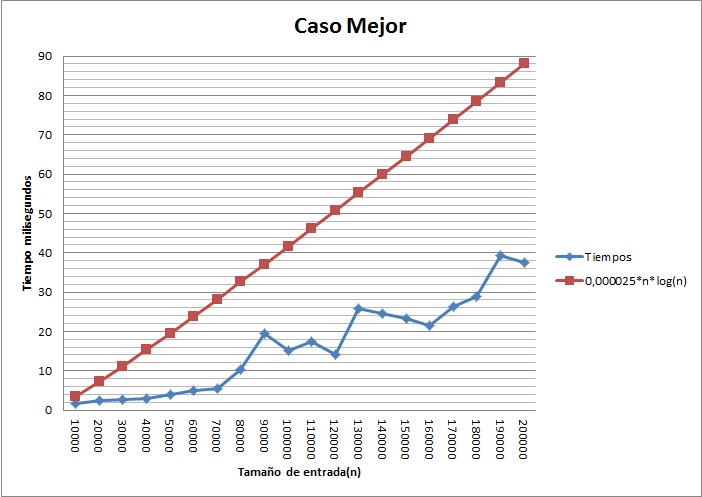
\includegraphics[scale=0.50]{imagenes/MejorCasoEj2.jpg}
  \end{center}
  \caption{ejemplo}
\end{figure}

El primer grafico del ejercicio 2, es el que compara al mejor caso con n*log(n), y en este grafico se puede ver claramente, que la curva de 
n*log(n) es una cota para los tiempos que se tomaron de lo que tarda en correr nuestro ejercicio para cotas cada vez mas grandes. Este grafico es importante mostrarlo, para que se vea que nuestro mejor caso, (que es mejor que el peor caso para todo n, visto del lado de complejidad de mejor y peor caso)
siempre esta acotado por n*log(n), que es siempre menor que n*n. Entonces aparte de la justificacion de la complejidad, habiendo tomado tiempos
no demuestra, pero apoya a la complejidad calculada.

\begin{figure}[H]
  \begin{center}
      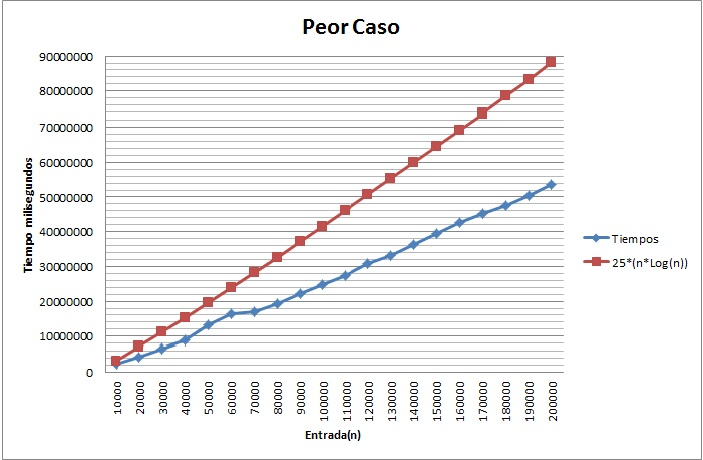
\includegraphics[scale=0.50]{imagenes/PeorCasoEj2.jpg}
  \end{center}
  \caption{ejemplo}
\end{figure}

El siguiente grafico, es el grafico de peor caso, comparado con n*log(n) que este es en realidad uno de los mas importantes, ya que tambien apoya nuestro calculo
de complejidad anterior, que decia que nuestro peor caso, para todo n = la sumatoria de i= 1 hasta n step 2 de log(i/2) + la sumatoria de i = 2 hasta n step 2 de 3*log(i/2)
Entonces al haber graficado n*log(n) por una constante, se puede ver que cae siempre por arriba de nuestros tiempos, y se puede ver que a la larga (mirando para n mayores)
la diferencia es cada vez mas grande.

\begin{figure}[H]
  \begin{center}
      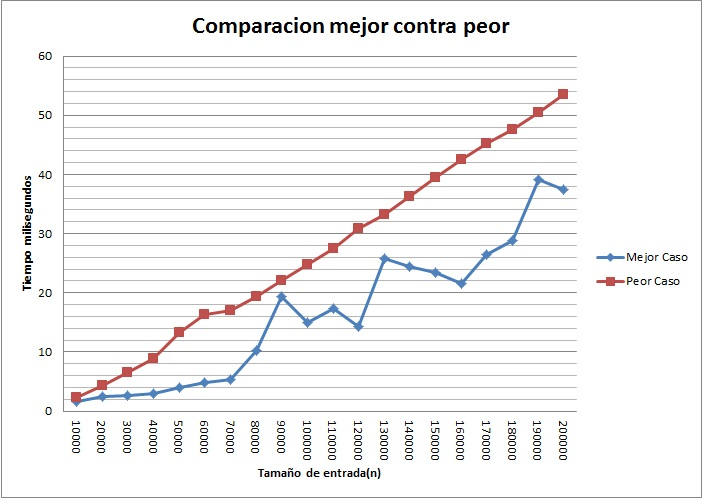
\includegraphics[scale=0.50]{imagenes/ComparacionEj2.jpg}
  \end{center}
  \caption{ejemplo}
\end{figure}

Y el grafico de mejor y peor caso, es simplemente para apoyar a la complejidad, ya que se puede ver facilmente que el mejor caso nunca puede ser mayor al peor.
Ya que la complejidad del mejor caso es la sumatoria de i = 1 hasta n de log(i/2) y la de peor caso mencionada varias veces es: la sumatoria de i= 1 hasta n step 2 de log(i/2) + la sumatoria de i = 2 hasta n step 2 de 3*log(i/2)
Entonces veremos que el grafico es coherente a lo recien dicho.



%\textbf{completar!}
\begin{figure}[H]
  \begin{center}
      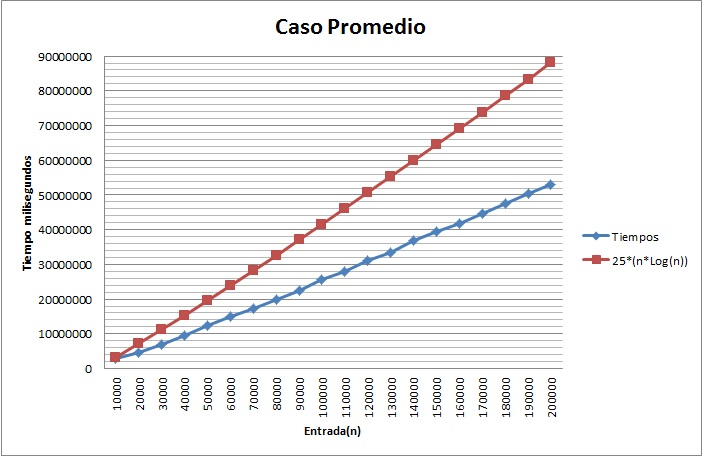
\includegraphics[scale=0.50]{imagenes/CasoPromedioEj2.jpg}
  \end{center}
  \caption{ejemplo}
\end{figure}

El ultimo grafico, es el del promedio, que este fue tomado agarrando numeros pseudoaleatorios, de la clase Random, de java. Este es el que probablemente
sea el mas parecido a como serian los tiempos tomados de cuando se use el programa, ya que si no buscas caer en un caso en particular, probablemente vayas cayendo en ambos casos, y 
no siempre en el mejor, ni siempre en el peor caso. Que como esta acotado por el peor caso, tambien es menor a n*log(n) y por consecuencia, a n al cuadrado.

\subsection{Validación}

Para validar el algoritmo, utilizamos casos de test, los cuales son una expansión de los test de la cátedra, para los cuales conocemos cual es la salida. En el archivo que contiene las instancias de entrada se llama $ Ej2\_validacion.in $, y los resultados esperados en $ Ej2\_validacion.out $.


\newpage
\section{Problema 3}
\subsection{Descripción del problema.}



%\vspace*{0.3cm}

%\textbf{completar!}
%\begin{figure}[htb]
%  \begin{center}
%      \includegraphics[scale=0.25]{imagenes/ejemplo.jpg}
%  \end{center}
%  \caption{ejemplo}
%\end{figure}

El objetivo de este algoritmo es obtener una configuración para una ronda de niñas exploradoras óptima, en el sentido de que la suma de las distancias entre los pares de amigas sea mínima. Cada niña es representada por una letra distinta. Se tiene como entrada del algoritmo a desarrollar para este problema una serie de niñas con algunas de sus respectivas amigas. El algoritmo debe obtener estos valores desde una archivo de texto con un formato como se puede ver en el siguiente ejemplo:


\begin{verbatim}
a bcde;b acde;c abde;d abc;e abc
a bcd;b ae;c ad;d ac;e b
a fb;b gc;d gc;f agh;e hd
x yz
\end{verbatim}

En cada linea tenemos una instancia distinta. A partir de la misma podemos obtener la cantidad total de exploradoras, y para cada una cuales son sus todas amigas. Hay que aclarar que cuando una niña es amiga de otra, esta ultima también es amiga de la primera. En la entrada solo tenemos para algunas exploradoras cuales son algunas de sus amigas. Cada string separado por un ';' indica las amistades, por ejemplo ''a bcde;'' significa que 'a' es amiga de 'b','c','d','e'. Para tener la totalidad de las amistades, se deben considerar las amistades reciprocas de las dadas originalmente, es decir también considerar que 'b', 'c', 'd' y 'e' son amigas de 'a'. Para una linea(instancia), no hay repetidos para los primeros carácteres de los string separado por un ';'. Por ejemplo para ''a dbe;b acde;c abde;d abc;e abc'',los primeros carácteres son 'a', 'b', 'c', 'd', 'e', y no se repiten. Tampoco se repiten las amistades, es decir que por ejemplo no es valida una entrada que tenga ''a dbed;'', o una misma exploradora tenga amistad consigo misma, por ejemplo ''a abed;''

Se tendrá una salida como se puede ver a continuación:

\begin{verbatim}
2 abdce
2 abecd
3 abcfgdhe
1 xyz
\end{verbatim}

Donde cada linea es la salida de una instancia, el numero representa la distancia máxima entre dos amistades dentro de la ronda. Esta última es representada por el string que sigue al número. Se considera que el primer y ultimo carácter estan unidos en la ronda.

\subsection{Desarrollo de la idea y pseudocódigo.}

%\vspace*{0.3cm}

%\textbf{completar!}

%\begin{codebox}
%\Procname{$\proc{ejemplo_de_pseudocodigo}(x,y)$}
%\li \Return $\id{solucion}$
%\end{codebox}

Para obtener la suma mínima de la distancia entre las amistades, se puede no considerar la reciproca de cada amistad. Por ejemplo si tenemos que ''a'' es amiga de ''b'', lo cual implica que ''b'' es amiga de ''a'', se puede solo considerar la distancia entre ''a'' y ''b'', pero no la reciproca.

El algoritmo del problema consiste en para cada linea del archivo de entrada, obtener un string, separarlo cada '';''. Cada elemento del arreglo contiene un string con información sobre las amistades. A partir del arreglo, construimos una lista enlazada de tuplas $ < $carácter, conjunto$ < $carácter$ > > $, donde cada elemento del conjunto es un carácter que tiene una amistad con el de la primera coordenada de la tupla. Esta lista enlazada se llama $ amistades $ en el algoritmo implementado. Para que no halla amistades repetidas, en el proceso de construir esta lista, antes de guardar un carácter en el conjunto, nos fijamos si ya había en la lista enlazada una amistad entre el elemento a agregar y la primera coordenada, en ese caso no agregamos.

Además creamos un un conjunto con los caracteres distintos que van apareciendo, para esto aprovechamos el Set de la biblioteca de java. Para utilizar la tupla se utilizara una clase especialmente creada, llamada Pair, que implementa las funcionalidades básicas de la misma. 

Luego llamamos a una función $minimaSuma$, que utilizando la lista con las amistades sin duplicados, un arreglo de char con los elementos del conjunto de exploradoras, y un arreglo de char pasado por parámetro donde se ira almacenando la palabra(representa una ronda) de suma mínima. Esta a su vez llama a la función $ minimaSumaAux $ la cual es una función que recursivamente ira calculando la suma entre las distancias de las amistades para cada permutación, para lo cual utiliza una función específica $ calcularSumaDistancias $. Para ir almacenando la suma mínima a medida que se recorren las permutaciones, se utiliza una instancia de una clase creada por nosotros llamada Entero. La misma contiene un solo campo de tipo int, y funciones get y set para manipularla. Como es un objeto, se pasa por referencia, y trabaja como un puntero que almacena un valor.
En caso de obtener una permutación con igual suma de distancias que la mínima actual, se preguntará si el es menor alfabéticamente, y en ese caso se almacenara.

Para calcular la distancia entre dos exploradoras, se toma la mínima distancia, entre las dos posibles direcciones. Para esto se calcula la distancia en un sentido, y para saber la distancia en el otro sentido se resta a la cantidad de exploradoras el anteriormente obtenido.

A continuación podemos ver los pseudocódigos de las funciones $minimaSuma$ y $ minimaSumaAux $.

\begin{codebox}
\Procname{$\proc{minimaSuma}(char[]\  original, list<caracter, Set<caracter>> \ amistades), char[]\  palabraMinima) $}
	\li \textbf{int} tam $ \leftarrow $ original.longitud
	\li \textbf{char[]} primero= new char[tam];
	\li primero[0]= original[0];
	\li \textbf{Entero} sumaMinima= new Entero(Integer.MAX_VALUE);	
	\li //lamamos a la funcion minimaSumaAux con un nivel de cero
	\li $minimaSumaAux(original, primero,0,tam,sumaMinima,palabraMinima, amistades);$
\end{codebox}

 La siguiente es la aridad de la función  $ minimaSumaAux :$ 
 
\begin{verbatim}
minimaSumaAux(char[] original, char[] agregado, int  nivel,int tam,
 Entero sumaMinima, char[] palabraMinima, List<Pair<Character, Set<Character> > > amistades)
\end{verbatim}
 
En la misma $original $ es un arreglo de char con los caracteres originales con los que se deben formar todas las permutaciones posibles. El método para efectuar esto llevado a cabo por $minimaSumaAux$ consiste en cada ''nivel'', es decir cuando la variable nivel tiene cierto valor, agregar un nuevo carácter de original a $ agregado $, y hacer todas las permutaciones posibles entre este nuevo carácter creando un nuevo arreglo de char para cada una de ellas. Por ejemplo si tenemos 

\begin{verbatim}
original=abcdef	         	agregado= cef		        nivel=3
\end{verbatim}

Hay que aclarar que $ agregado $ tiene el tamaño de la cantidad total de exploradoras, aunque solo esta completo con caracteres hasta índice nivel. Le agregamos a $agregado$ la letra indicada por nivel , en este caso la ''d'', de la siguiente manera agregado[nivel]= ''d''. Hacemos todas las permutaciones entre esta ultima y las anteriores letras de $agregado$, obteniendo.

\begin{verbatim}
cefd cedf cdfe defc
\end{verbatim}

Creamos un arreglo de char para cada una , aunque del tamaño de la cantidad de exploradoras.

Luego para cada permutación, y para el agregado modificado, llamamos recursivamente a $minimaSumaAux$, con los mismos parámetros, pero con el nivel aumentado en una unidad, y en lugar de agregado los nuevos arreglos de char. Este método nos permite crear un único arreglo de char por cada permutación.

Se ejecuta recursivamente el algoritmo hasta que llega al caso base que es cuando el nivel es el tamaño de las exploradoras, en ese caso se llama a la función $ calcularSumaDistancias $ que calcula la suma entre las distancias entre las amistades, y en caso de que la permutación en cuestión tenga menor suma, o igual, pero alfabéticamente menor, se almacenan estos valores en los objetos sumaMinima(Entero) y palabraMinima(arreglo de char).

Finalmente se llama a la función $calcularMaxDist$, que calcula todas las distancias, entre todas las amistades, y va almacenando el valor máximo.

\newpage

\subsection{Análisis de complejidad.}

%\vspace*{0.3cm}

%\textbf{completar!}

Se calcularan las complejidades en base los parámetros de entrada cantidad de exploradoras, denotado por $ n $ , y cantidad de amistades, denotado por $ a $.

En el siguiente fragmento se analiza la complejidad para una instancia, antes de llamar a $minimaSuma$

\begin{lstlisting}
String[] amistadesPuntoComa= line.split(";"); 
//es una funcion de la libreria	de java, no se encontro la documentacion con su complejidad, pero se puede estimar en a lo sumo el tamanio del string al cuadrado, con lo que seguro es menor a O( (na)^2 ).
String relacion;
List<Pair<Character, Set<Character>>> amistades= new LinkedList<Pair<Character, Set<Character>>>();
				
//contiene a las exploradoras
Set<Character> exploradoras= new LinkedHashSet<Character>()
				
for(int i=0;i<amistadesPuntoComa.length;i++){// tiene como mucho n iteraciones
	relacion=amistadesPuntoComa[i]
	char nuevoCaracter = relacion.charAt(0)
	exploradoras.add(nuevoCaracter)
	// al agregar algo a un conjunto, tiene un costo del tamanio del mismo, asi q es menor o igual a O(n)
					
//en este par guardamos todos los caracteres que se relacionan con nuevoCaracter
	Pair<Character,Set<Character> > nuevoPar =new Pair<>(nuevoCaracter,new HashSet<Character>())
	amistades.add(nuevoPar)
//empezamos desde indice dos para evitar el espacio
	for(int j=2;j<relacion.length();j++){
						
		char caracter_relacion= relacion.charAt(j)
		exploradoras.add(caracter_relacion) // nueva mente al agregar algo a un conjunto, tiene un costo del tamanio del mismo, asi q es menor a O(n)
								
		boolean hayQueGuardar=true
		for(Pair<Character,Set<Character> >  par: amistades){// seguro tiene menos o igual a n iteraciones		
			if(par.getFirst()==caracter_relacion){
				Set<Character> relaciones_caracter= par.getSecond()						
				for(Character c:relaciones_caracter){// seguro tiene menos o igual a n iteraciones							
					if(c==nuevoCaracter){
						hayQueGuardar=false
						break
						}
				}				
				break
			}					
		}// tenemos un costo de menor o igual a O(n^2) este ciclo
		if(hayQueGuardar){
			nuevoPar.getSecond().add(caracter_relacion) //puede tener un costo como mucho de O(n) ya que agregamos algo a un conjunto
		}
	}
} al finalizar este ciclo tenemos un costo menor o igual a O(n^3*a^2)

//con un iterador pasamos el Set de exploradoras a un arreglo de char, con un costo de O(n)
char[] original= new char[exploradoras.size()]
Iterator<Character> itExpl= exploradoras.iterator()
int indice=0
while(itExpl.hasNext()){
	original[indice]=itExpl.next()					
	indice++
}
					
int tam= original.length
char[] palabraMinima= new char[tam]	
minimaSuma(original,amistades,palabraMinima)
\end{lstlisting}

Se tiene un costo menor o igual a $ O(n^{3}a^{2}) $ antes de llamar a $ minimaSuma $ por lo que el orden de la complejidad estará dominado por esta ultima función.

A continuación se detallan algunas de las funcione auxiliares utilizadas, con sus complejidades. 

\begin{lstlisting}

	public static int calcularDistancia(char[] instancia, int desde,char c){
		
		int dist=0
		int indice=desde
		 for(int j=0;j<instancia.length;j++){ // a lo sumo n iteraciones	 
			 dist++ 
			 indice++ 
			 indice %=instancia.length;
			 
			 if(instancia[indice]==c){
				 break
			 }	 
		 } 
		 return Math.min(dist, instancia.length-dist);
	}

\end{lstlisting}

Como la función utiliza a lo sumo n iteraciones, tiene un costo de O(n).


\begin{lstlisting}
public static int calcularSumaDistancias(char[] instancia, List<Pair<Character, Set<Character> > > amistades){
		
	int sumaDistancia=0
	int distanciaCaracter
	for(int i=0;i<instancia.length;i++){ //exactamente n iteraciones
		char c1= instancia[i]
		for(Pair<Character, Set<Character> > par: amistades){ //a lo sumo n iteraciones
			if(par.getFirst()==c1){
				for(char c: par.getSecond()){// a lo sumo n iteraciones
					distanciaCaracter= calcularDistancia(instancia,i,c) // costo a lo sumo O(n)
					sumaDistancia +=distanciaCaracter					
				}//costo de cada iteracion de este ciclo O(n)
			break	
			}				
		}
	}
	return sumaDistancia
}
\end{lstlisting}

Como el tercer for anidado del anterior fragmento solo se ejecuta para una de las n iteraciones del segundo for(debido al condicional if) los podemos considerar a los dos como uno solo con un costo igual al del tercer for sumado a un costo de $O(n)$ en peor caso. La cantidad total de veces que se ejecuta el cuerpo del tercer for es menor o igual a la cantidad de relaciones, y como el costo de cada un es $O(n)$, tenemos un costo total de $O(na)$. Como se mensionó, para cada iteración del primer ciclo, además del costo del tercer ciclo, tenemos un costo de O(n), con lo que tenemos un costo adicional de $O(n^2)$. De esta forma podemos decir que el costo de esta función es $O(n^2+na)$ o $O(an^2)$



%Como esta es una función que se utilizara para cada permutación, se podría mejorar la implementación para reducir la complejidad de la misma, estableciendo previamente una relación entre cada carácter y sus amistades especificadas en la lista enlazada, de manera de poder acceder en forma directa para cada carácter a sus amistades.



El siguiente es un fragmento del código de la función $ minimaSuma$, en el mismo podemos ver que la complejidad esta dominada por $ minimaSumaAux $.
\begin{lstlisting}
	private static void minimaSuma(char[] original, List<Pair<Character, Set<Character> >  > amistades, char[] palabraMinima){
		
		int tam= original.length	
		char[] primero= new char[tam]
		primero[0]= original[0]
		Entero sumaMinima= new Entero(Integer.MAX_VALUE)
		minimaSumaAux(original, primero,0,tam,sumaMinima,palabraMinima, amistades)
}
\end{lstlisting}

En el siguiente fragmento podemos encontrar el código de la función $ minimaSumaAux $.

\begin{lstlisting}

	private static void minimaSumaAux(char[] original, char[] agregado, int nivel,int tam, Entero sumaMinima, char[] palabraMinima, List<Pair<Character, Set<Character> >  > amistades){
		
		if(nivel==tam-1){// caso base
						
			int sumaDistancia= calcularSumaDistancias(agregado, amistades);//O(a*n^2)
			if(sumaDistancia<sumaMinima.getValor()){// este if en peor caso O(n)
				
				sumaMinima.setValor(sumaDistancia)	
				for(int j=0;j<tam;j++){//O(n)
					palabraMinima[j]=agregado[j]
				}//costo de O(n)		
			}	
			if(sumaDistancia==sumaMinima.getValor() && esMenor(agregado,palabraMinima)){// tambien este if en peor caso O(n)
				
				//guardamos la palabra minima
				for(int j=0;j<tam;j++){
					palabraMinima[j]=agregado[j]
				}
			}
			return; // tenemos un costo de caso base de O(a*n^2) en peor caso
		}
		
		
		int nuevoNivel=nivel+1
		char nuevoCaracter =original[nuevoNivel]

		List<char[]> permut = new LinkedList<char[]>()
		agregado[nuevoNivel]=nuevoCaracter
		permut.add(agregado)
		for(int i=0;i<=nuevoNivel-1;i++){
			
			char[] aAgregar = new char[tam]// a lo sumo alojar un arreglo en memoria, un costo de O(n)
			for(int j=0;j<=nuevoNivel;j++){	
				aAgregar[j]=agregado[j]		
			}//costo de O(nuevoNivel)
			
			swap(aAgregar,i,nuevoNivel)	//costo O(1)
			permut.add(aAgregar)
			
		}//costo de O(nivel*n) antes de llamar recursivamente

		for(char[] arr: permut){
			//se llama recursivamente a la misma funcion, pero esta esta mas cerca del caso base
			minimaSumaAux(original, arr,nuevoNivel, tam, sumaMinima, palabraMinima, amistades);		
		}
		
		permut.clear()
		
	}
\end{lstlisting}


Para calcular la complejidad, si en lugar de hacerlo con una ecuación de recurrencia, se tiene en cuenta que el caso base se ejecuta para cada una de las permutaciones posibles, que el costo de crear y ordenar cada arreglo de char es $ O(n) $, y que hay exactamente uno por permutación, como hay$ n! $ permutaciones, tenemos un costo de $ O(n!(n+an^2)$, lo que es equivalente a $ O(an!n^2)$. 

Para obtener la complejidad $ T_1(n) $ de la función $ minimaSumaAux $, podemos plantear una función $ T(nivel,n) $ que calcula la cantidad de operaciones elementales por nivel que realiza la anterior función, en el sentido de que para el nivel n se consideran todas las operaciones de nivel superior. Decimos que una operación elemental esta en un cierto nivel si es llamada desde una función $ minimaSumaAux $ con ese parámetro en el campo nivel. De esta manera para obtener la complejidad $ T_1(n) $, evaluamos $T(0,n)$. Pero para esta nueva función, podemos plantear una ecuación de recurrencia.

\begin{equation*}
T(nivel,n) = \left\lbrace
\begin{array}{c}
 (nivel+2)T(nivel+1)+(nivel+1)n) \ \ \ si \ \ \ \  nivel< n-1 \\
  an^2  \  \ \ \  \ si \ \ \ \  nivel==n-1 \\
\end{array}
\right.
\end{equation*}

Para obtener  $T(0,n)$, podemos expandir la evaluación:
\begin{equation*}
\begin{array}{c}
 T(0,n)=2T(1,n)+n=2(3T(2,n)+2n)+n=3!T(2,n)+2^{2}n+n= \\
  = 3!(4T(3,n)+3n)+2^{2}n+n=4!T(3,n)+3^{2}2!n+2^{2}1!n+n=\cdots\\
 \cdots = n!(n^2a) + \sum_{i=0}^{n-1} (i+1)^{2}i! n  \\
\end{array}
\end{equation*}

Seguro podemos acotar a la función de complejidad resultante por una de la forma $ n!p(n)a $, con p un polinomio, por lo que su complejidad seguro pertenece a $O(n!p(n)a)$.

Como antes de llamar a la función $ minimaSuma $ se tenía un costo de $ O(n^{3}a^{2})$, tenemos un costo total para el algoritmo del ejercicio 3 que pertenece a $ O(n!p(n)a^2)$.

El orden de la complejidad es estrictamente menor que $ O(a^2n^n)$, ya que vale que $ O(n!p(n)) $ con p un polinomio, es estrictamente menor que $ O(n^n) $.

Finalmente se llama a a función $calcularMaxDist$, para calcular la máxima distancia entre pares de amigas. Su costo computacional se calcula igual que para la función $calcularSumaDistancias$, y es el mismo.

 Como para todas las instancias de entrada se hacen todas las permutaciones y para cada una se calcula la suma para ver si es menor a la suma acumulada, no hay grandes diferencias entre peor caso y mejor caso.
 
 
 



\subsection{Correctitud}

Para garantizar que nuestro algoritmo es solución del problema, se tiene que cumplir que se evalue $ calcularSumaDistancias $ para todas las permutaciones posibles. Para esto se tiene que cumplir que la forma en que las construimos abarca todos los casos. En el siguiente ejemplo, podemos ver que para cada nivel de la función $minimaSumaAux$, se obtienen todas las permutaciones posibles


\begin{figure}[H]
\centering
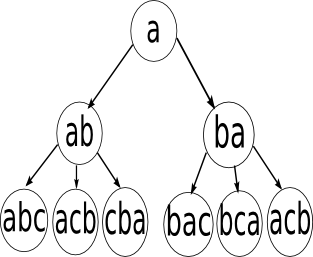
\includegraphics[scale=0.8]{imagenes/ej3Correctitud.png}
\caption{Permutaciones posibles para }
\label{256value}
\end{figure}



Podemos describir que lineas generales el método, el cual se explico en la sección anterior, consiste en tomar en cada paso, todas las permutaciones generadas en el paso anterior, agregarle un nuevo caracter a todas, y construir todas las secuencias resultantes de intercambiar el nuevo caracter con los demás caracteres, incluyendo la que solo le agrega al final el nuevo.

Demostraremos por inducción en la cantidad de pasos, que el método llevado a cabo por nuestro algoritmo, genera todas las permutaciones.

Para esto demostraremos dos proposiciones previas:

\begin{itemize}
\item En el paso $ n $ tenemos secuencias de $ n $ elementos.
\item En el paso $ n $ tenemos $ n! $ secuencias.
\item Las permutaciones obtenidas en cada paso son todas distintas.
\end{itemize}

Con estas tres ultimas podemos, y usando que la cantidad de permutaciones de una secuencia de $ n $ elementos es $ n! $, podemos demostrar que en cada paso se tiene la cantidad maxima de permutaciones para un dado tamaño de secuencia. Se tiene la máxima cantidad, si tiene $ n! $, y no tiene secuencias repetidas.

La primera proposición se puede probar en forma trivial por inducción en la cantidad de pasos.

Probemos también por inducción la segunda proposición. 

El caso base se cumple de manera trivial para $ n=1 $, ya que tenemos una secuencia, lo cual coincide con $1! $. 

Veamos el paso inductivo, es decir que si vale en el paso $ n $, entonces vale en el paso $ n+1 $. 

Sabemos que en el paso $ n $ hay $ n! $ secuencias(HI), veamos que en el paso $ n+1 $ hay $ (n+1)! $ secuencias. Par cada una de las secuencias de $ n $ elementos, en el paso $ n+1 $ construimos las $ n+1 $ instancias que surgen de intercambiar el nuevo carácter agregado con un solo carácter de los anteriores, incluyendo la secuencia en que no se intercambia el nuevo carácter agregado. Como se tienen $ n+1 $ secuencias, para cada una de las secuencias del paso anterior, y en este último había $ n! $, tenemos un total de $ (n+1)n! $ en el nuevo nivel, es decir $ (n+1)! $, como queríamos probar.

La tercer proposición, nuevamente se probara por inducción, pero se utilizará fuertemente el siguiente lema:
\bigskip

\textbf{Lema 1:} Si tengo un conjunto de secuencias distintas, con el último carácter igual, al generar todas las posibles secuencias que resultan de permutar el último carácter, con alguno(solo uno) de los restantes, inclulléndose, tenemos que todas las obtenidas son distintas.
\bigskip

Procedemos a demostrar el lema, utilizando el absurdo. Supongamos que entre dos secuencias distintas hacemos un intercambio entre el último carácter, y algún índice(puede ser distinto entre ambas), obteniendo dos secuencias iguales.

Separamos en casos:

\begin{itemize}
\item Si el ultimo carácter se intercambia con índices distintos,tenemos que estas nuevas secuencias difieren en el índice donde se inserto el último carácter, abs.
\end{itemize}


\begin{itemize}
\item Si el ultimo carácter se intercambia con índices iguales
	\begin{itemize}
		\item En caso de que en las palabras el elemento del índice con que se intercambia es distinto, tenemos que las nuevas secuencias difieren en el último carácter, abs 
		\item En caso de que sean iguales los caracteres(y el índice), como las secuencias originales eran distintas, debe existir algún otro índice en que difieran en un carácter. Este índice no fue modificado, así que las secuencias siguen siendo distintas.
	\end{itemize}
\end{itemize}

Ahora procedemos a probar inductivamente la tercer proposición. El caso base es trivial ya que para un paso, todas las secuencias son distintas, ya que hay una sola. Para probar el paso inductivo, utilizamos el lema anterior.
\subsection{Validación}

Se corroboro que pasen los test de la cátedra. Se verifico que se ejecute correctamente para un archivo de entrada especialmente preparado con casos borde llamado $ Ej3\_validacion.in $, y se observo que la salida era aceptable. Para cada instancia de test ejecutada, se verifico imprimiendo por pantalla que el arreglo de tuplas llamado $ amistades $ contenía los caracteres esperados. Se imprimió por pantalla la suma mínima obtenida, y se verificó que coincidía con la suma de distancias calculada a mano. Las funciones para imprimir esto en pantalla se encuentran comentadas.

Para verificar que se probaron todas las permutaciones posibles, se utilizo una lista enlazada en la cual se guardaban todas las instancias. Se verificó que la misma no tenia repetidos, y que su cantidad era n!. La misma se llamaba $ recolectadas $ y se encuentra comentada en el código, para utilizarla se debe además utilizarla de parámetro en $minimaSumaAux$, ya que que en el código entregado no se encuentra esta funcionalidad. No obstante no se puede utilizar esta lista en caso de que la cantidad de caracteres sea mayor a cierto numero, porque se gastaría mas memoria del que soporta la maquina. En este sentido se corroboro que para la ultima instancia de $ Ej3\_validacion.in $ la maquina no se queda sin memoria, verificándose que el programa no se gastan mas de 230 Mb, y no tarda mas de dos horas en ejecutarse. En caso de utilizar la lista enlazada para esta instancia, la maquina se queda sin memoria.


\newpage
\subsection{Experimentación}

En una experiencia se dejo fijo el ''a'' en 7, y se vario el ''n'' desde 8 a 13. Se corrió dos veces(para tomar promedio) el algoritmo, utilizando la clase $Ejercicio3$, con una pequeña modificación para medir tiempos e imprimirlo en pantalla, la cual fue borrada posteriormente. En la figura~\ref{aCte} podemos visualizar los resultados.

\begin{figure}[H]
  \begin{center}
      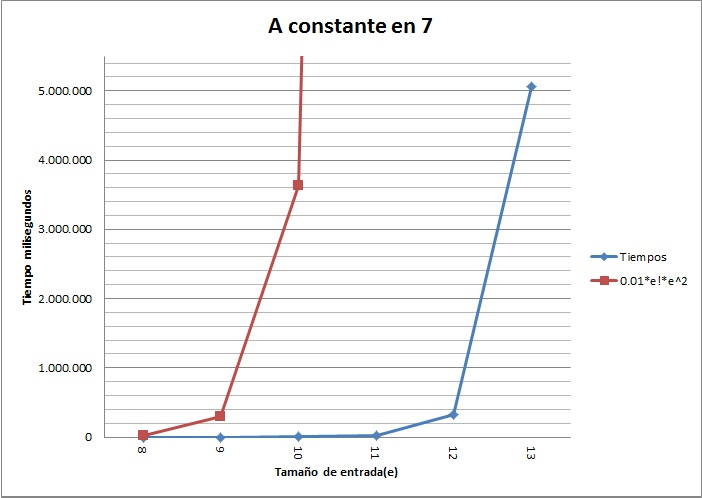
\includegraphics[scale=0.75]{imagenes/GraficoEj3Aacotado7.jpg}
  \end{center}
  \caption{En azul encontramos el gráfico de tiempos obtenidos en función de n, en rojo el gráfico de una función con un comportamiento similar}
  \label{aCte}
\end{figure}

También se constato que el tiempo para un ''n'' de 14, el tiempo era mayor a 15 hs. En base a estos resultados, esperamos que para una cantidad de exploradoras mayor, el tiempo esperado sea mucho mayor aun.

Para otra experiencia se dejo fijo el ''n'' en 12, y se vario el ''a''. Nuevamente se corrió dos veces, para tomar promedio, el algoritmo, utilizando la clase $Ejercicio3$, con una pequeña modificación para medir tiempos e imprimirlo en pantalla. En la figura~\ref{nCte} podemos ver los resultados obtenidos.

\begin{figure}[H]
  \begin{center}
      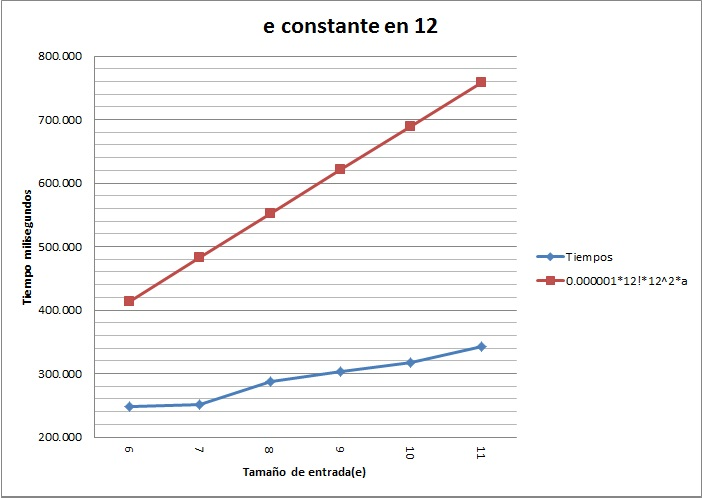
\includegraphics[scale=0.75]{imagenes/GraficoEj3Ncte12.jpg}
  \end{center}
  \caption{En azul encontramos el gráfico de tiempos obtenidos en función de n,en rojo el gráfico de una función con un comportamiento similar}
  \label{nCte}
\end{figure}

Según nuestro calculo de complejidad, al no tener la especificación de la función $ split $ de la clase $ String $ de java, no sabiamos si la complejidad final dependía de $ a $ o de $a^2$. Sin embargo como el termino $a^2$, no multiplica a $ n! $, no tiene relevancia en la complejidad final. Con los resultados obtenidos podríamos decir que es lineal, los puntos podrían ser ajustados por una función lineal de una cierta pendiente y ordenada al origen.



\newpage



\newpage
\section{Apéndice 1: Otras secciones relevantes del código}
En esta sección, adjuntamos parte del código correspondiente a la resolución de cada problema
que consideramos más \textbf{relevante}.

\subsection{Código del Problema 1}

\begin{lstlisting}
public class Telegrafo {
	public static int maximasEstacionesConectadas( int[] estaciones , int mCable ) {
		
		int desde=0;
		int hasta=0;
		int cantEstacionesConectadas=0;
		int cantidadDeEstacionesMaxima=0;
		boolean mePase=false;
		while(hasta<estaciones.length-1){
			while(hasta<estaciones.length && estaciones[hasta]-estaciones[desde]<=mCable){
				hasta++;
				mePase=true;
			}
			if(mePase) {
				hasta--;
				mePase=false;
			}
			
			cantEstacionesConectadas=desde-hasta==0 ? 0 : hasta-desde+1;
			cantidadDeEstacionesMaxima=Math.max(cantidadDeEstacionesMaxima, cantEstacionesConectadas);
			desde++;
		}
		return cantidadDeEstacionesMaxima;
	}
}
\end{lstlisting}

%\vspace*{0.5cm}

%\begin{lstlisting}
%int main(){
%  return 0;
%}
%\end{lstlisting}

\newpage
\subsection{Código del Problema 2}

\begin{lstlisting}
	public static List<Integer> obtenerMedianas(List<Integer> numeros_entrada){
		
		List<Integer> medianas= new ArrayList<Integer>();//aca retorno las medianas parciales
		
		Comparator<Integer> inversoComparador =Comparator.<Integer> reverseOrder();
		
		PriorityQueue<Integer> mitadMenores = new PriorityQueue<Integer>(inversoComparador);//es un maxHeap

		PriorityQueue<Integer> mitadMayores= new PriorityQueue<Integer>(); // es un minHeap
		
		
		for(Integer e:numeros_entrada ){
			
			//primero inserto el nuevo elemento donde corresponda
			
			if(mitadMenores.isEmpty()){
				mitadMenores.add(e);
			}else if(mitadMayores.isEmpty()){
						
				Integer primero= mitadMenores.peek();
				
				if(primero>e){
					mitadMayores.add(mitadMenores.poll());
					mitadMenores.add(e);
				}else{
					mitadMayores.add(e);
				}
				
				
			}else if(e>mitadMayores.peek()) {
				mitadMayores.add(e);
			}else {
				mitadMenores.add(e);
			}
			
			//luego rebalanceo para que queden con igual cantidad, o en caso de impar que halla uno mas en la izquierda
			
			if(mitadMayores.size()>mitadMenores.size()){
				
				mitadMenores.add(mitadMayores.poll()); //poll no solo devueve la raiz, tambien la elimina del heap
				
			}else if(mitadMenores.size() - mitadMayores.size()>1){
				
				mitadMayores.add(mitadMenores.poll());
				
			}
			
			Integer aAgregar;
			
			if (mitadMenores.size() == mitadMayores.size()) {
				
				aAgregar= (mitadMenores.peek() + mitadMayores.peek()) / 2;
				
			} else {
				
				aAgregar= mitadMenores.peek();
				
			}
			
			medianas.add(aAgregar);
		
		}
		
		
		return medianas;
	}
	
\end{lstlisting}

%\vspace*{0.5cm}

%\newpage
%\subsection{Código del Problema 3}

%\begin{lstlisting}
%int main(){
%  return 0;
%}
%\end{lstlisting}

%\vspace*{0.5cm}

%\begin{lstlisting}
%int main(){
%  return 0;
%}
%\end{lstlisting}




\end{document}
